\section{Implementation}
\label{sec:implementation}

\begin{figure}[t!]
	\centering
	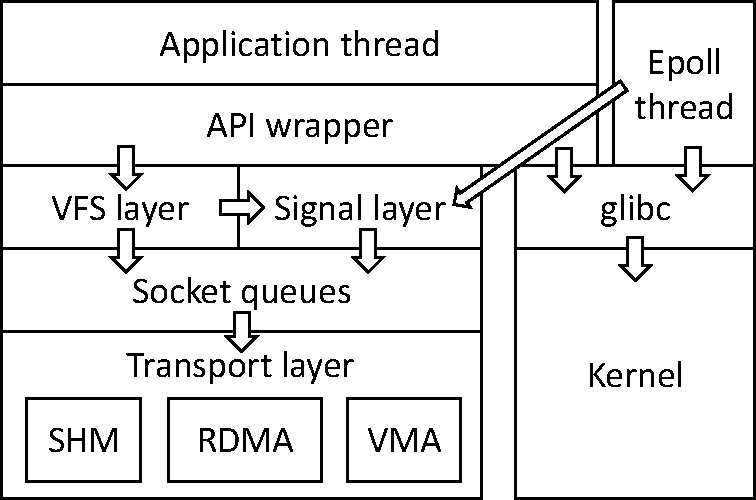
\includegraphics[width=0.25\textwidth]{images/libsd_architecture}
	\vspace{-5pt}
	\caption{Architecture of \libipc{}.}
	\label{fig:libsd-architecture}
\end{figure}


We implement \sys in three components: a user-space library \libipc{} and a monitor daemon with about 10K lines of C++ code, and a modified RDMA NIC driver to support zero copy.
As Figure~\ref{fig:libsd-architecture} shows, \libipc{} has a layered structure.

\RED{API wrapper -> FD remapping layer.}

\parab{FD allocation.}
FD remap table.

%For implementation, \libipc is divided to two parts: monitor and userspace library. Both parts are implemented in $\approx$5000 lines of C/C++ code. %We take advantage of C++ templates for different types of queues in our design.



%\subsection{Seamless system call hook}
%\label{subsec:syscall-hook}

%\parab{LD\_PRELOAD to intercept Linux APIs.}
%\libipc uses \textit{LD\_PRELOAD} environment variable in Linux to load a shared library and intercept the system call wrappers of GNU libc.

%\parab{Multiplex FD between kernel and \libipc{}.}
%Taking the idea of MegaPipe~\cite{han2012megapipe} and LOS~\cite{huang2017high}, we partition the FD space between \libipc and Linux kernel. Linux assigns FD from zero to $2^{30}-1$, while \libipc assigns FD from $2^{31}-1$ down to $2^{30}$.

\parab{Multiplex events between kernel and \libipc{}.}
The application polls events from both sockets and other \textit{kernel FDs} handled by Linux kernel.
A naive way to poll kernel events is to invoke the syscall (e.g. \texttt{epoll\_wait}) every time, which incurs high overhead because event polling is a frequent operation on virtually every send and receive.
%LOS~\cite{huang2017high} periodically invokes non-blocking \texttt{epoll\_wait} syscall with kernel FDs, which leads to a trade-off between delay and CPU overhead. Differently,
Differently, \libipc{} creates a per-process \textit{epoll thread} which invokes \texttt{epoll\_wait} syscall to poll kernel events. Whenever epoll thread receives a kernel event, it broadcasts the event to application threads via shared memory queues. Then the signal layer in \libipc{} will return such kernel events together with user-space socket events to the application.
%Note that Linux allows an event to be received by multiple threads.

%\textbf{Accelerate access to local storage.}
%Use SPDK and user-mode file system (cite). How to multiplex processes in accessing a file system? (1) directory and metadata go to monitor, (2) read/write within allocated area of a file: process self, (3) append or read/write outside allocated area: handled by master process of a shared file. Monitor pre-allocate free blocks to processes (batch allocation and free).
